\documentclass{beamer}

\beamertemplatenavigationsymbolsempty

\usepackage{amsmath}
\usepackage{amssymb}
\usepackage[absolute,overlay]{textpos}
\usepackage{braket}
\usepackage{graphics}
\usepackage{epstopdf}
\usepackage{tikz}
\usetikzlibrary{automata}

\DeclareMathOperator*{\argmin}{\arg\!\min}

\title{Part II Project - Progress Presentation}
\subtitle{Techniques for Separation of Harmonic Sound Sources}
\author[Will]{W. Simmons}
%\institute[Unis]{\inst{1} CompSci \\ Catz}
\date[08/02/2017]{8th February 2017}
%\subject{Computer Science}


\usetheme{Szeged}
\usecolortheme{beaver}
\setbeamertemplate{footline}[frame number]

%\linespread{1.4}

%\setbeamertemplate{logo}[C:/Users/Will/Pictures/fire\_music\_note\_by\_arghus-d5athqt.jpg]

%\logo{\includegraphics[height=1cm]{./CatzLogo.jpeg} \includegraphics[height=1cm]{./ChuLogo.png}}

\begin{document}

\frame{\titlepage}

%\begin{frame}
%
%\frametitle{Contents}
%
%\tableofcontents
%
%\end{frame}

%\section*{Directional time cues}
%\subsection*{}

\begin{frame}

\frametitle{Project Background}

Sound Separation is the inverse of mixing

\bigskip
\pause

Examples:

\begin{itemize}
\item Cocktail Party Problem

\item Unmixing music for analysis/sampling/remixing
\end{itemize}

\bigskip
\pause

Parameters:

\begin{itemize}
\item Uninformed

\item Harmonic sources

\item Known number of sounds
\end{itemize}

\end{frame}

\begin{frame}

\frametitle{Planned Work}

Michaelmas:

\begin{itemize}
\item Research Sinusoidal Modelling techniques and Non-Negative Matrix Factorisation

\item Obtain sample data and create test sets

\item Design and draft high-level solutions using both techniques
\end{itemize}

Christmas:

\begin{itemize}
\item Complete main implementation of solutions
\end{itemize}

Lent:

\begin{itemize}
\item Optimise feature weights for clustering

\item Obtain accuracy statistics over various test sets
\end{itemize}

Easter:

\begin{itemize}
\item Dissertation
\end{itemize}

\end{frame}

\begin{frame}

\frametitle{Current Progress}

Michaelmas:

\begin{itemize}
\item Research Sinusoidal Modelling techniques and Non-Negative Matrix Factorisation \checkmark

\item Obtain sample data and create test sets \checkmark

\item Design and draft high-level solutions using both techniques \checkmark
\end{itemize}

Christmas:

\begin{itemize}
\item Complete main implementation of solutions \checkmark
\end{itemize}

Lent:

\begin{itemize}
\item Optimise feature weights for clustering \checkmark

\item Obtain accuracy statistics over various test sets
\end{itemize}

Easter:

\begin{itemize}
\item Dissertation
\end{itemize}

\end{frame}

\begin{frame}

\frametitle{Example Results: Sinusoidal Modelling}

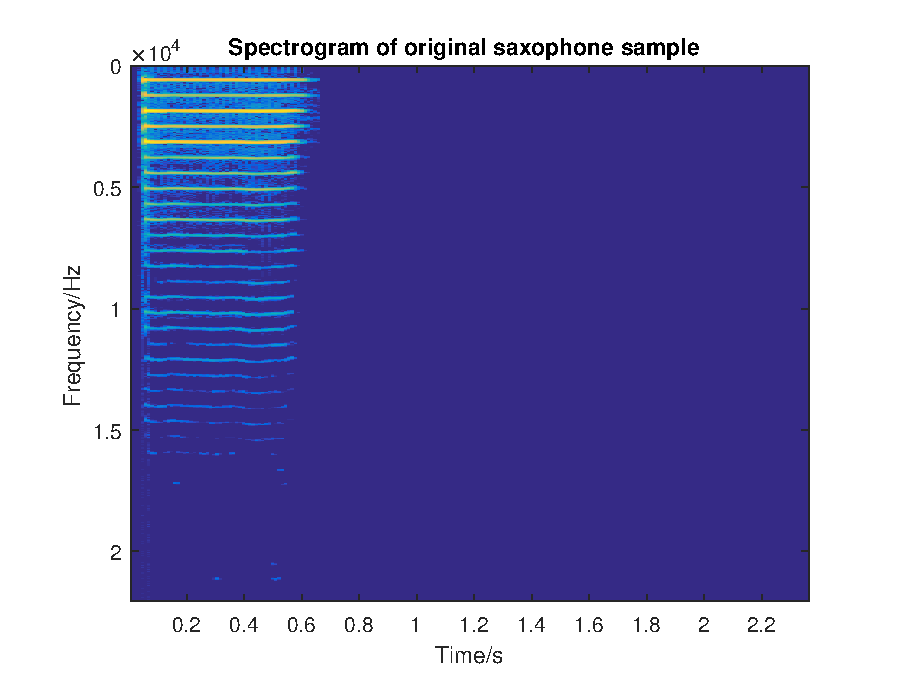
\includegraphics[width=0.5\linewidth]{./OriginalSaxophone.eps}
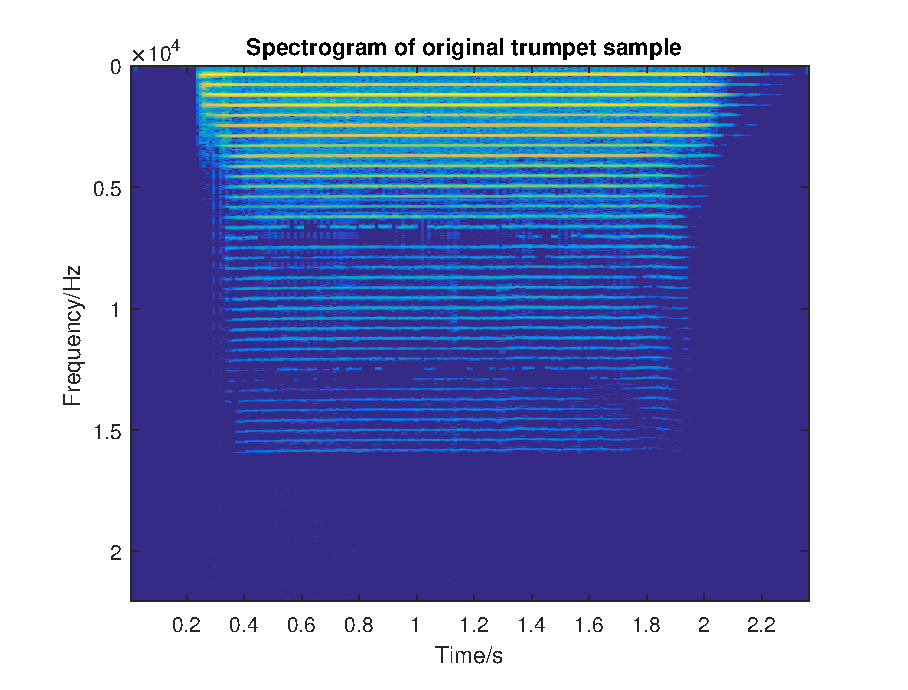
\includegraphics[width=0.5\linewidth]{./OriginalTrumpet.eps}

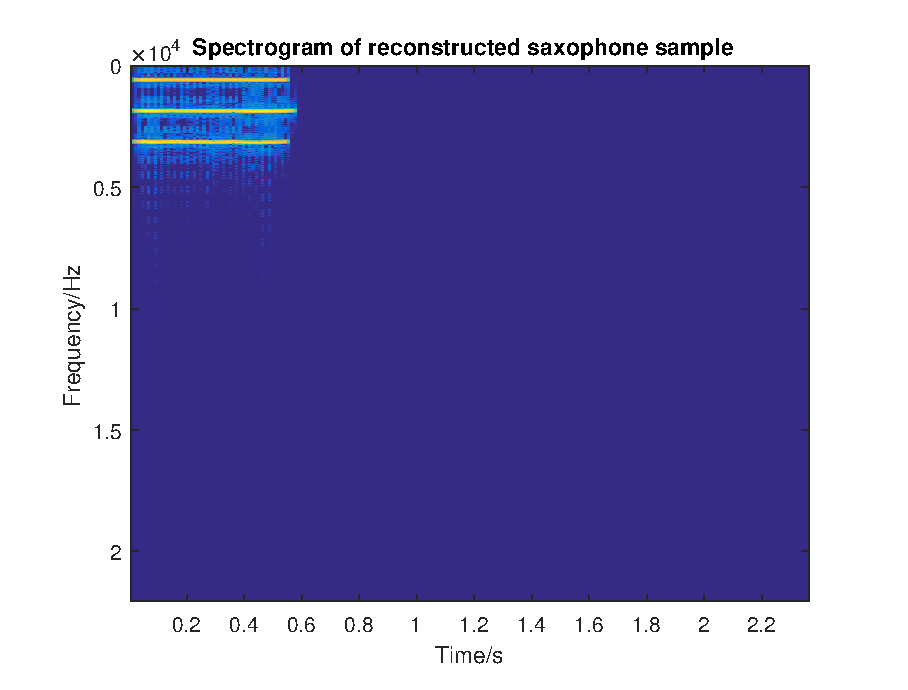
\includegraphics[width=0.5\linewidth]{./ReconstructedSaxophone.eps}
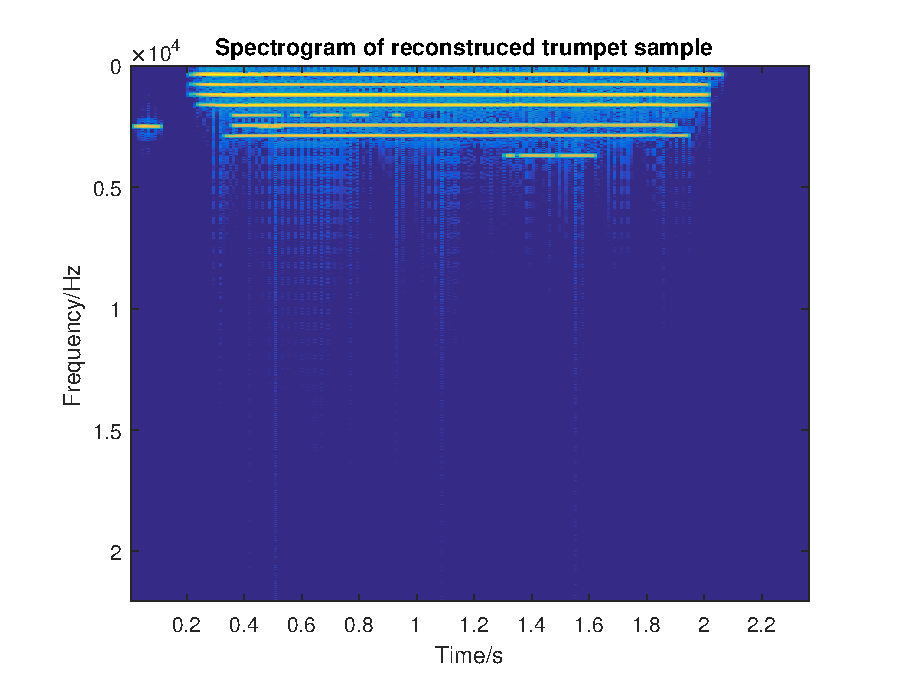
\includegraphics[width=0.5\linewidth]{./ReconstructedTrumpet.eps}

\end{frame}

\begin{frame}

\frametitle{Example Results: Sinusoidal Modelling (cont.)}

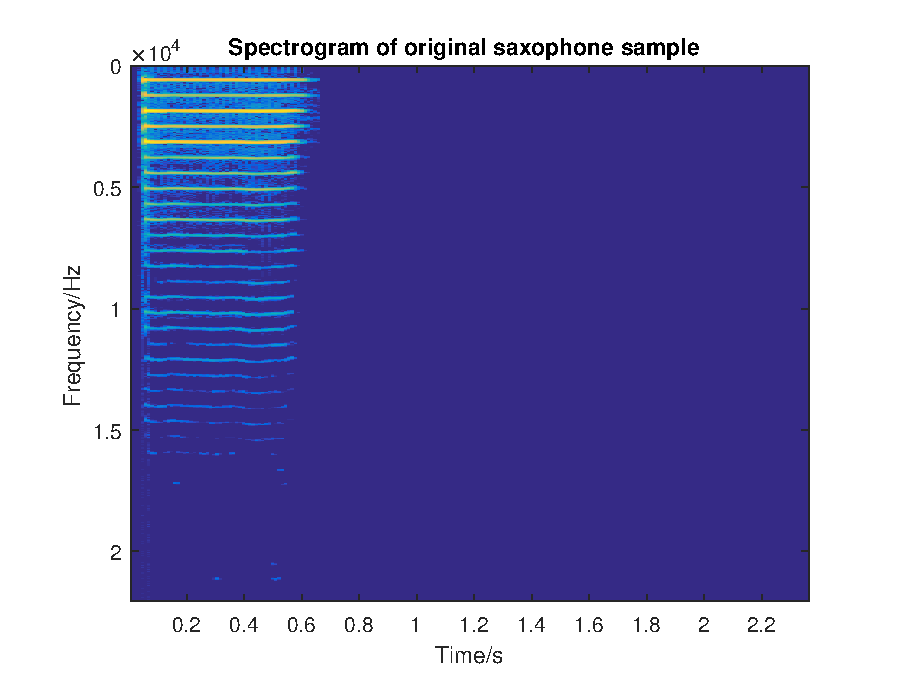
\includegraphics[width=0.5\linewidth]{./OriginalSaxophone.eps}
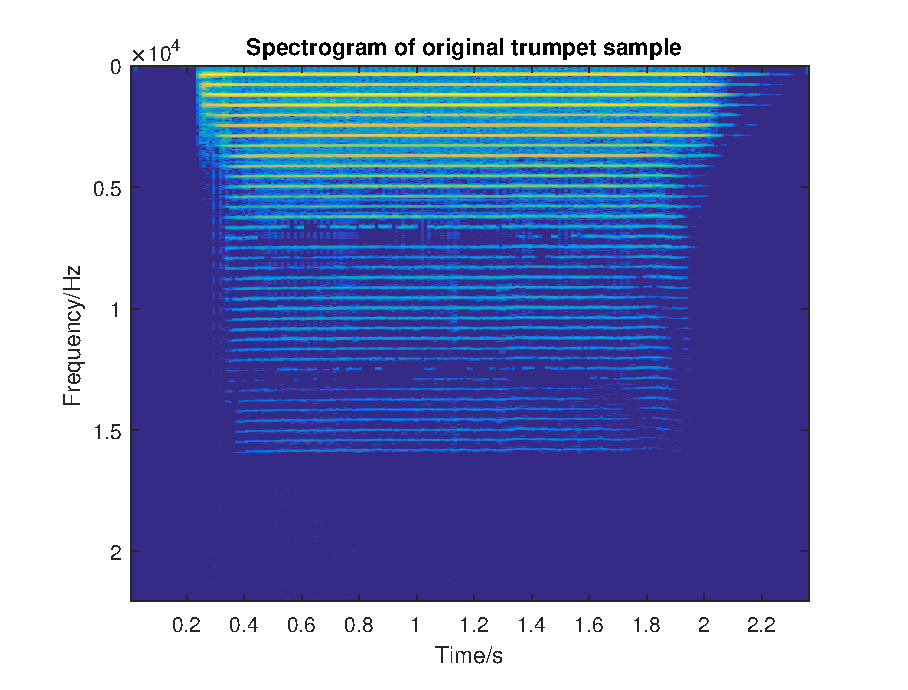
\includegraphics[width=0.5\linewidth]{./OriginalTrumpet.eps}

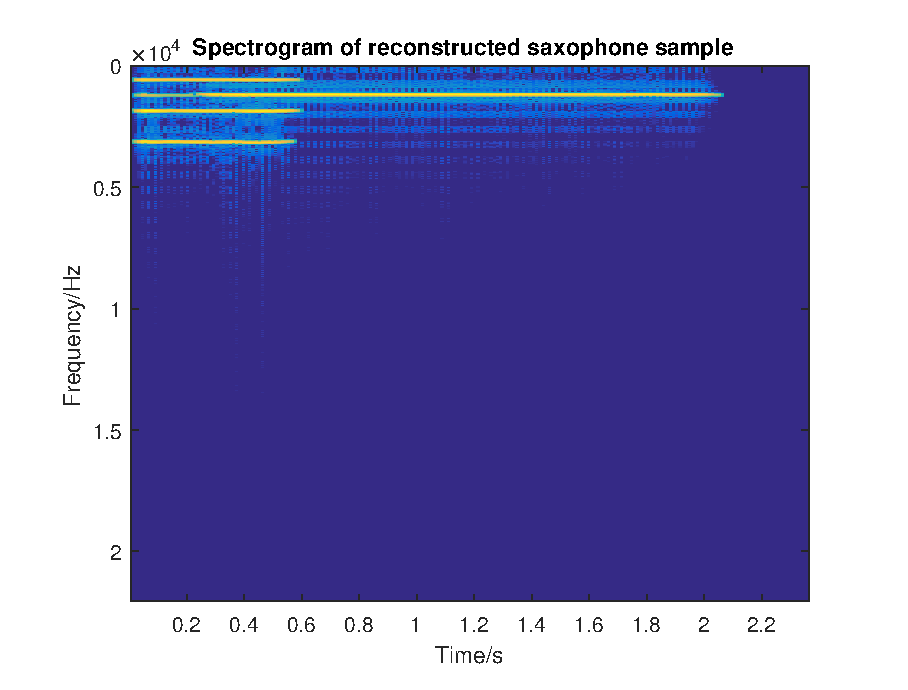
\includegraphics[width=0.5\linewidth]{./ReconstructedSaxophoneLowThreshold.eps}
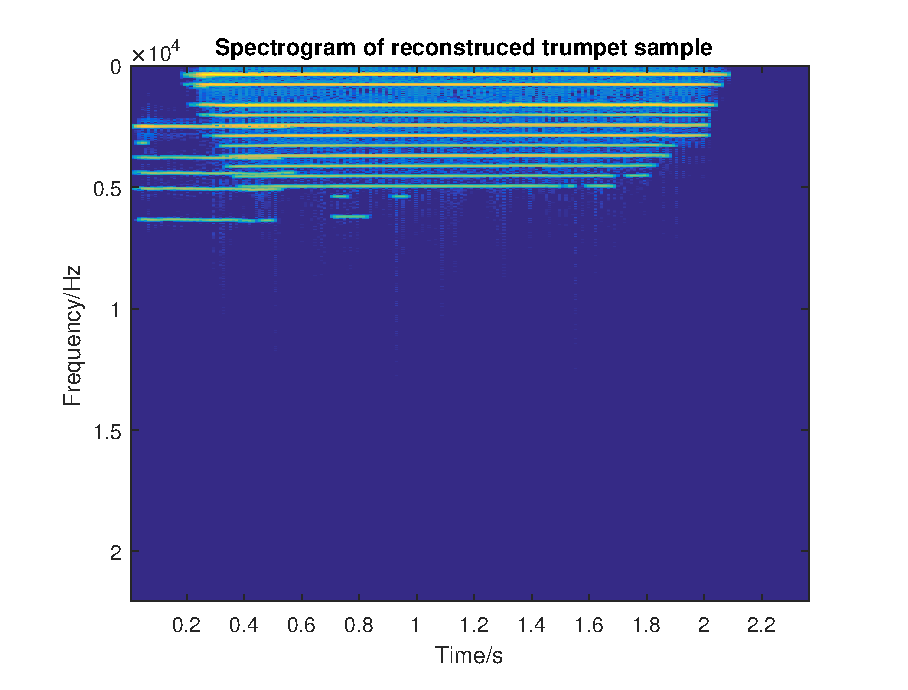
\includegraphics[width=0.5\linewidth]{./ReconstructedTrumpetLowThreshold.eps}

\end{frame}

\begin{frame}

\frametitle{Example Results: Sinusoidal Modelling (cont.)}

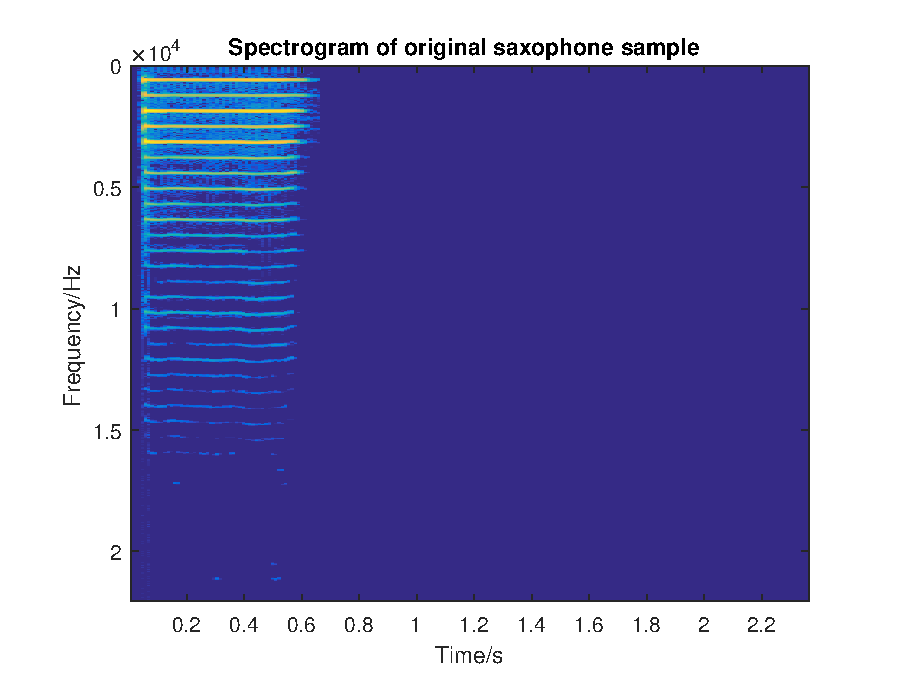
\includegraphics[width=0.5\linewidth]{./OriginalSaxophone.eps}
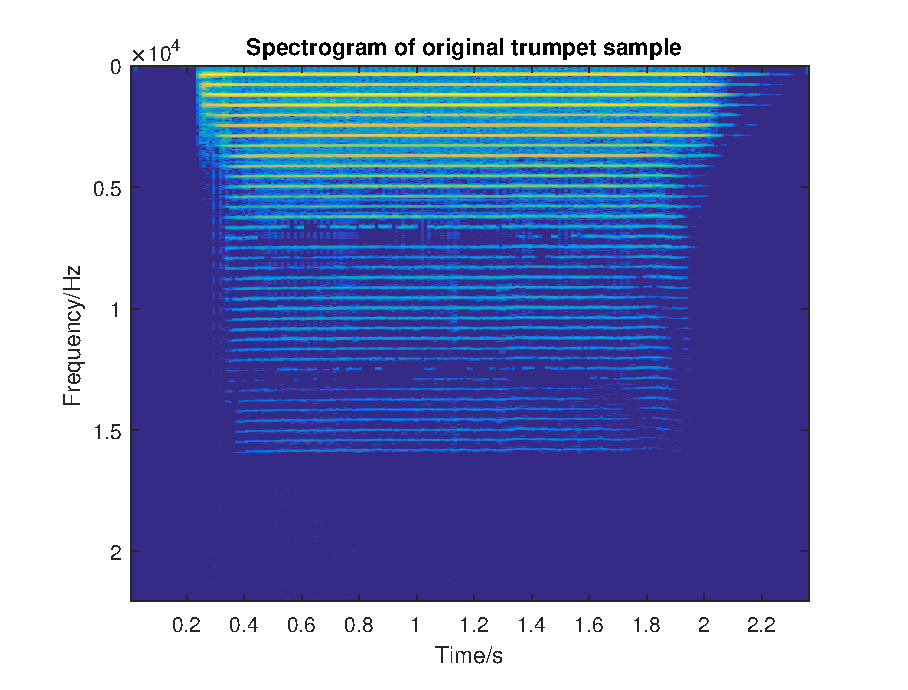
\includegraphics[width=0.5\linewidth]{./OriginalTrumpet.eps}

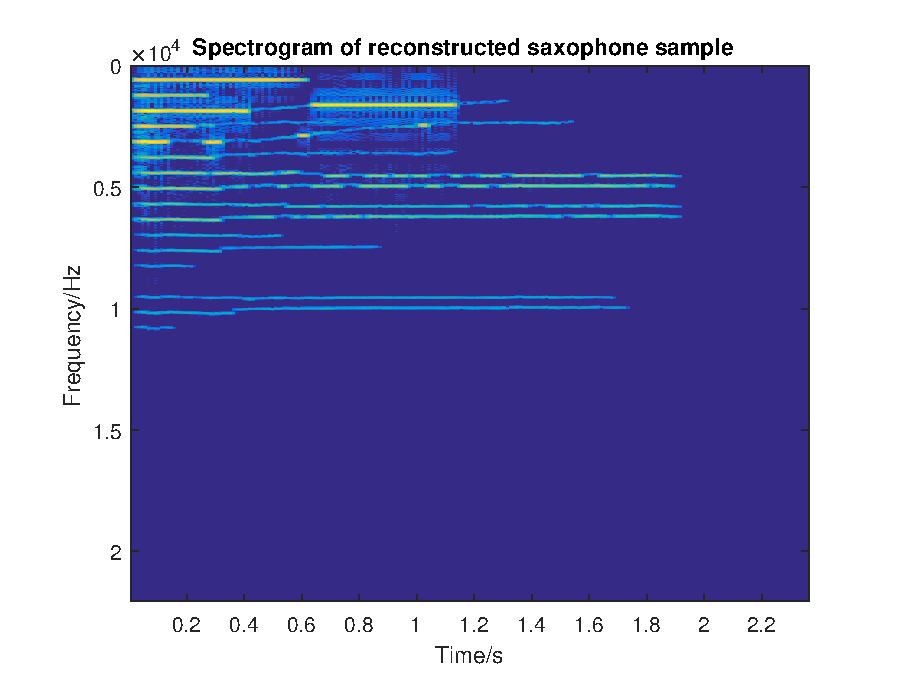
\includegraphics[width=0.5\linewidth]{./ReconstructedSaxophoneVLowThreshold.eps}
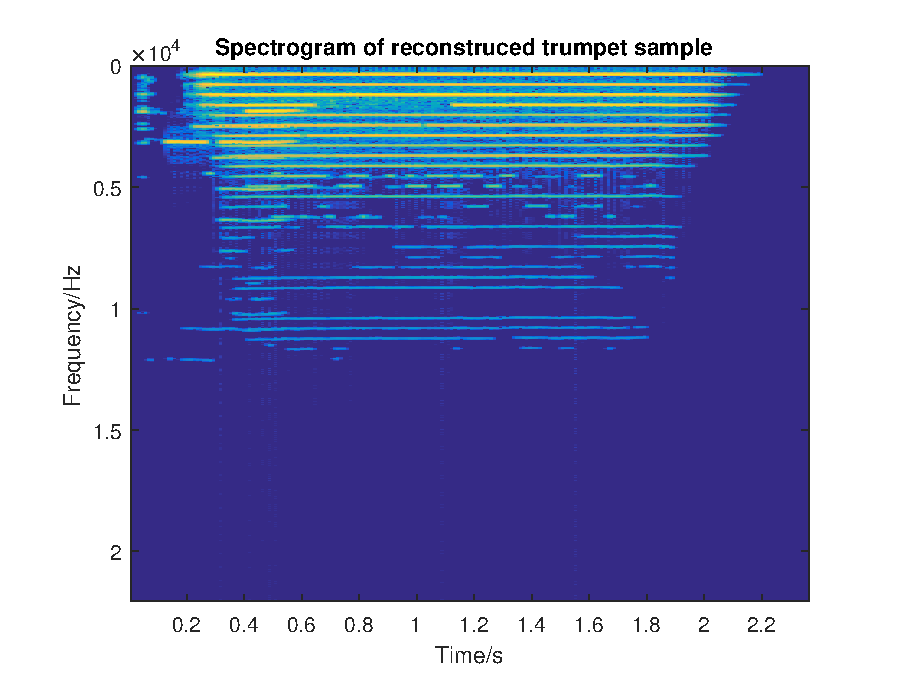
\includegraphics[width=0.5\linewidth]{./ReconstructedTrumpetVLowThreshold.eps}

\end{frame}

\begin{frame}

\frametitle{Example Results: Sinusoidal Modelling (cont.)}

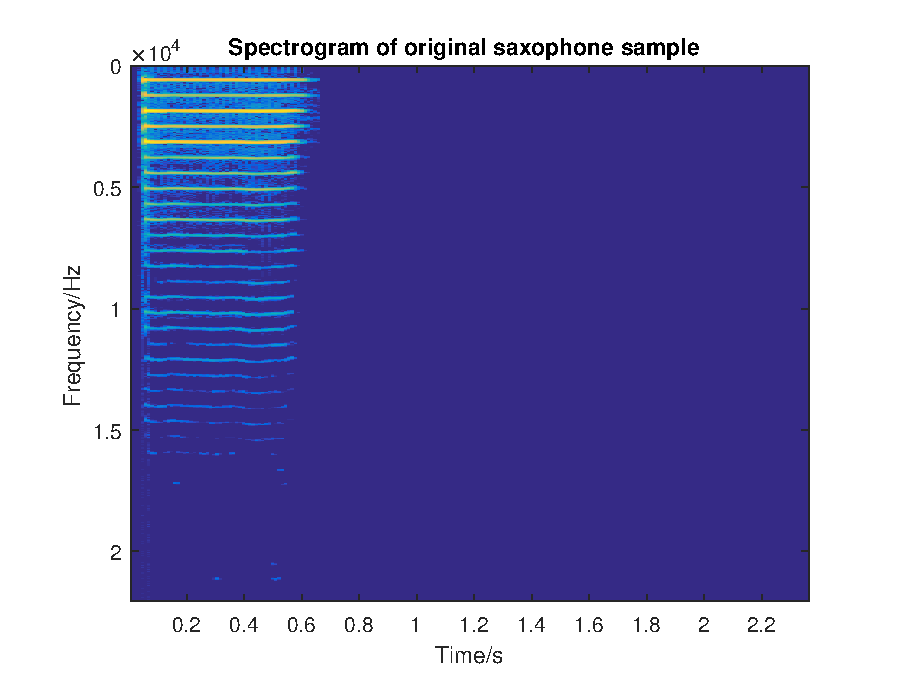
\includegraphics[width=0.5\linewidth]{./OriginalSaxophone.eps}
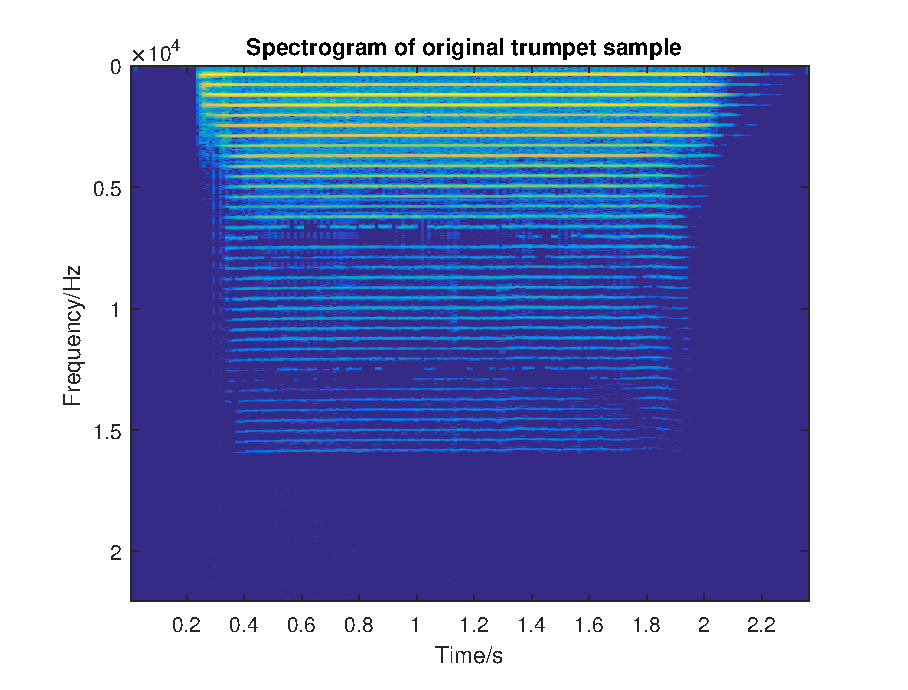
\includegraphics[width=0.5\linewidth]{./OriginalTrumpet.eps}

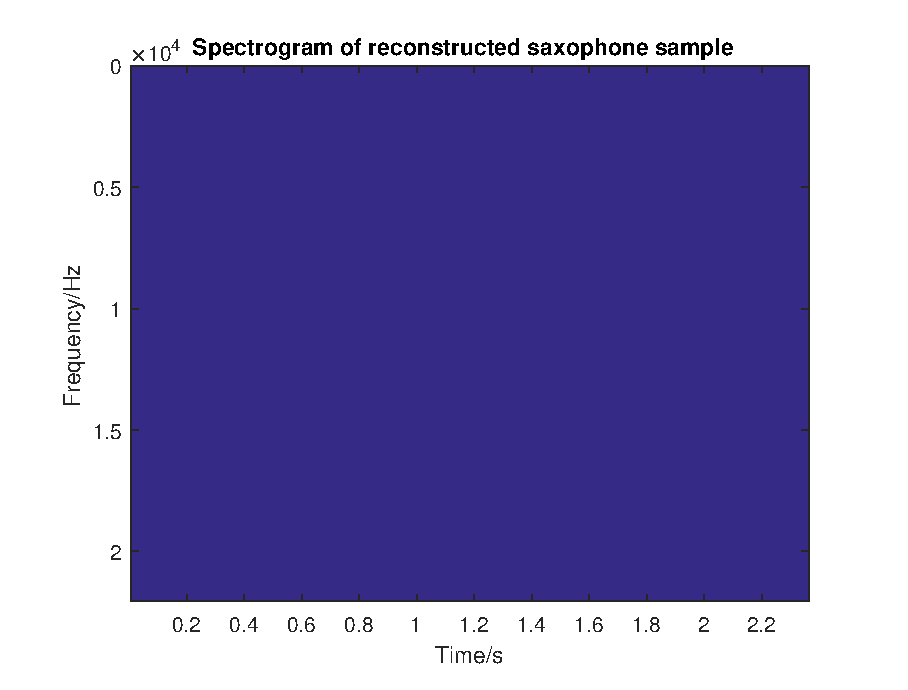
\includegraphics[width=0.5\linewidth]{./ReconstructedSaxophoneVVLowThreshold.eps}
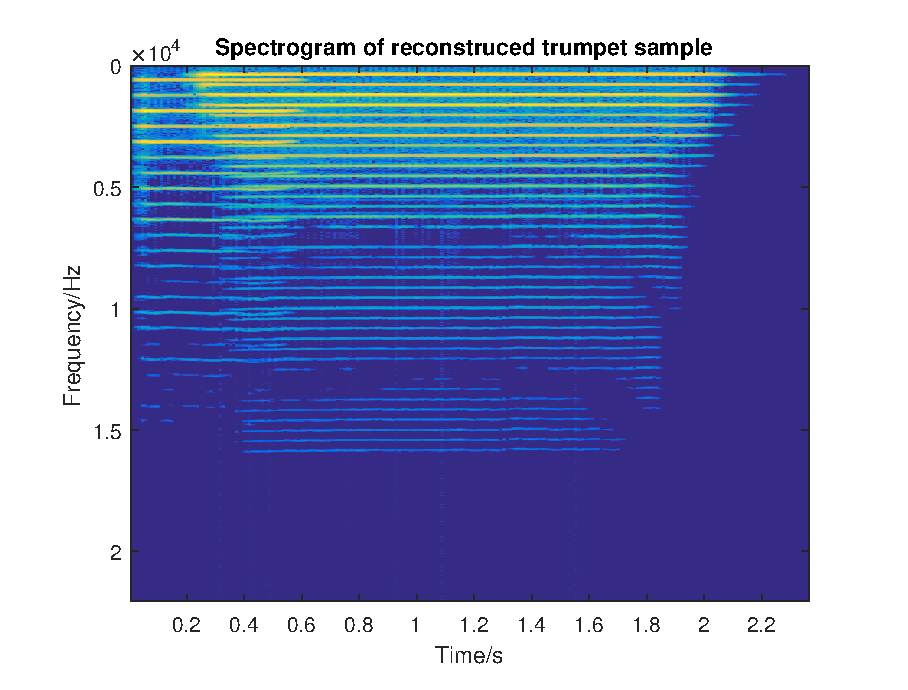
\includegraphics[width=0.5\linewidth]{./ReconstructedTrumpetVVLowThreshold.eps}

\end{frame}

\begin{frame}

\frametitle{Example Results: Sinusoidal Modelling}

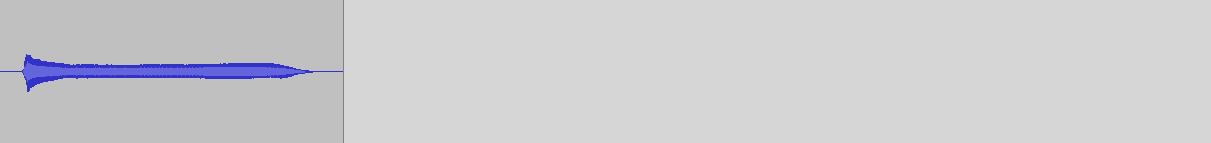
\includegraphics[width=0.8\linewidth]{./OriginalSaxophone.png}
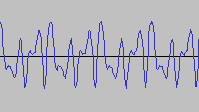
\includegraphics[width=0.17\linewidth]{./OriginalSaxophoneZoom.png}

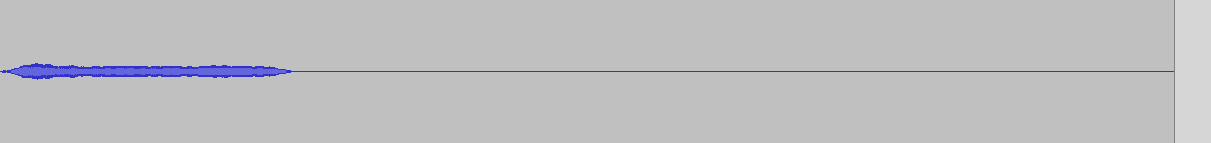
\includegraphics[width=0.8\linewidth]{./ReconstructedSaxophone.png}
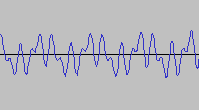
\includegraphics[width=0.17\linewidth]{./ReconstructedSaxophoneZoom.png}

\bigskip

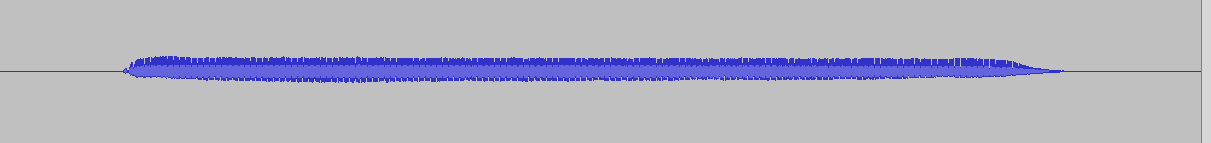
\includegraphics[width=0.8\linewidth]{./OriginalTrumpet.png}
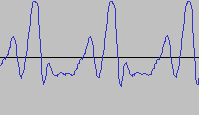
\includegraphics[width=0.17\linewidth]{./OriginalTrumpetZoom.png}

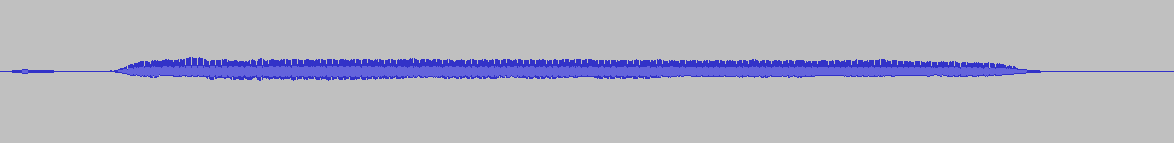
\includegraphics[width=0.8\linewidth]{./ReconstructedTrumpet.png}
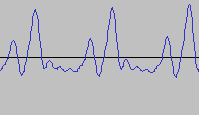
\includegraphics[width=0.17\linewidth]{./ReconstructedTrumpetZoom.png}

\end{frame}

\begin{frame}

\frametitle{Example Results: NMF}

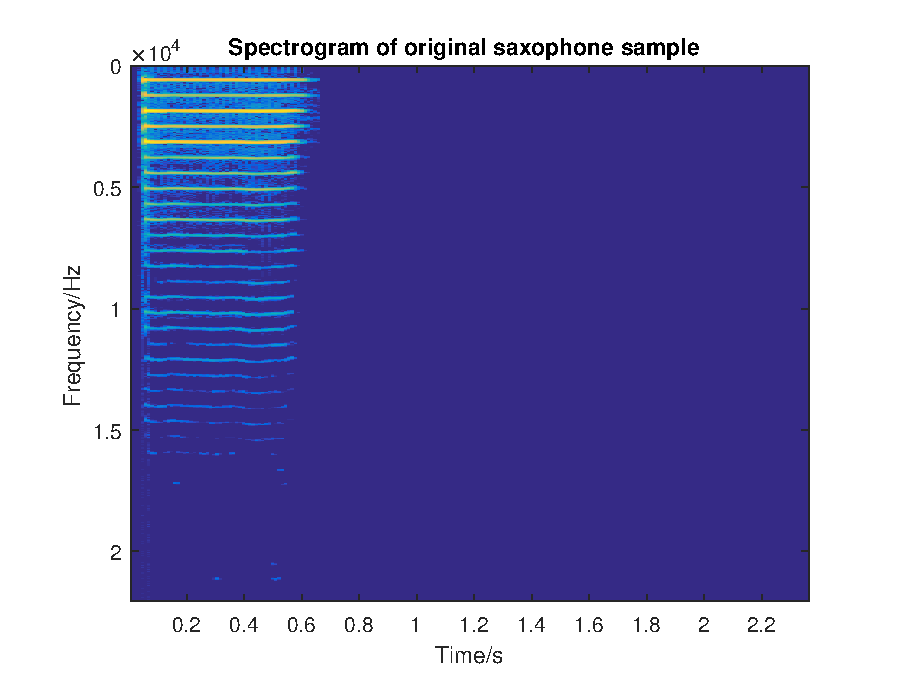
\includegraphics[width=0.5\linewidth]{./OriginalSaxophone.eps}
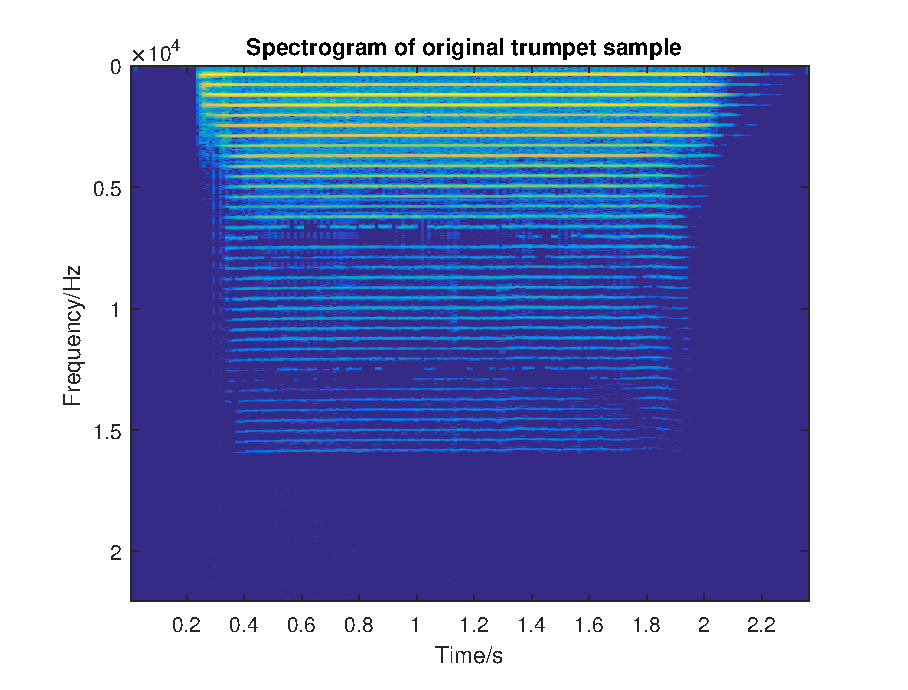
\includegraphics[width=0.5\linewidth]{./OriginalTrumpet.eps}

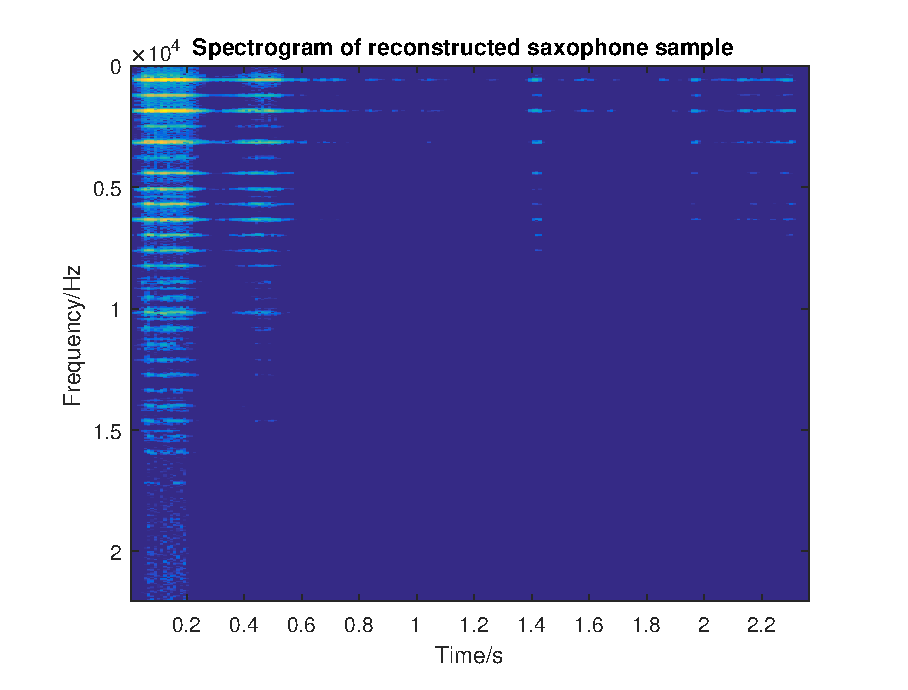
\includegraphics[width=0.5\linewidth]{./ReconstructedSaxophoneNMF2.eps}
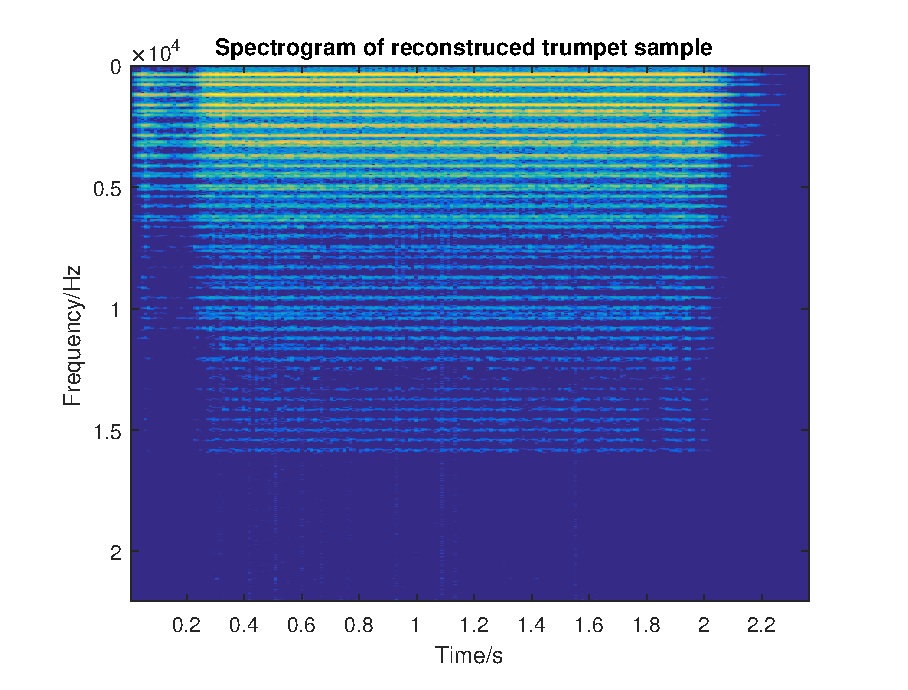
\includegraphics[width=0.5\linewidth]{./ReconstructedTrumpetNMF2.eps}

\end{frame}

\begin{frame}

\frametitle{Example Results: NMF (cont.)}

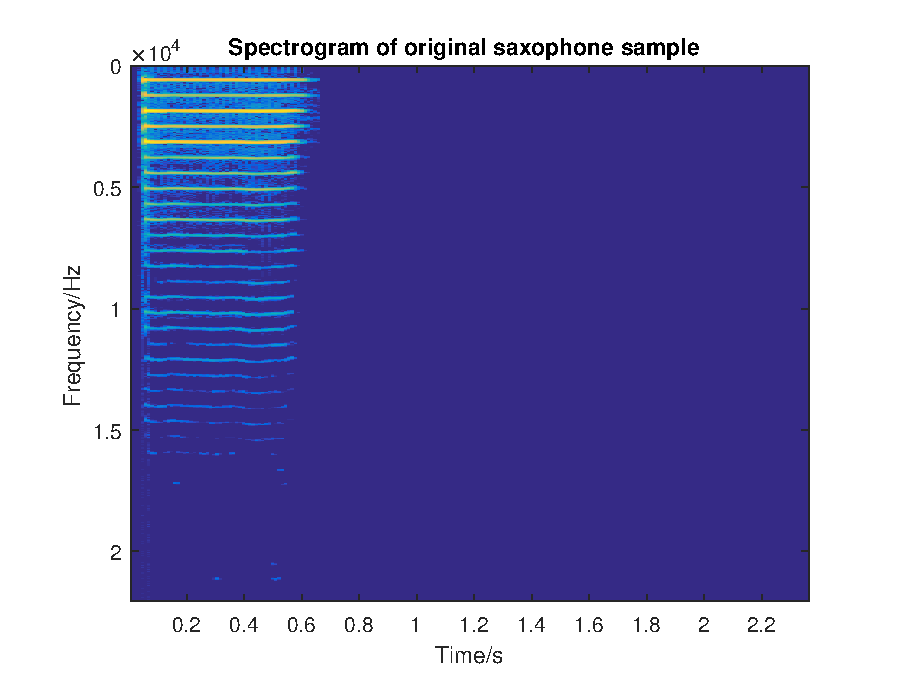
\includegraphics[width=0.5\linewidth]{./OriginalSaxophone.eps}
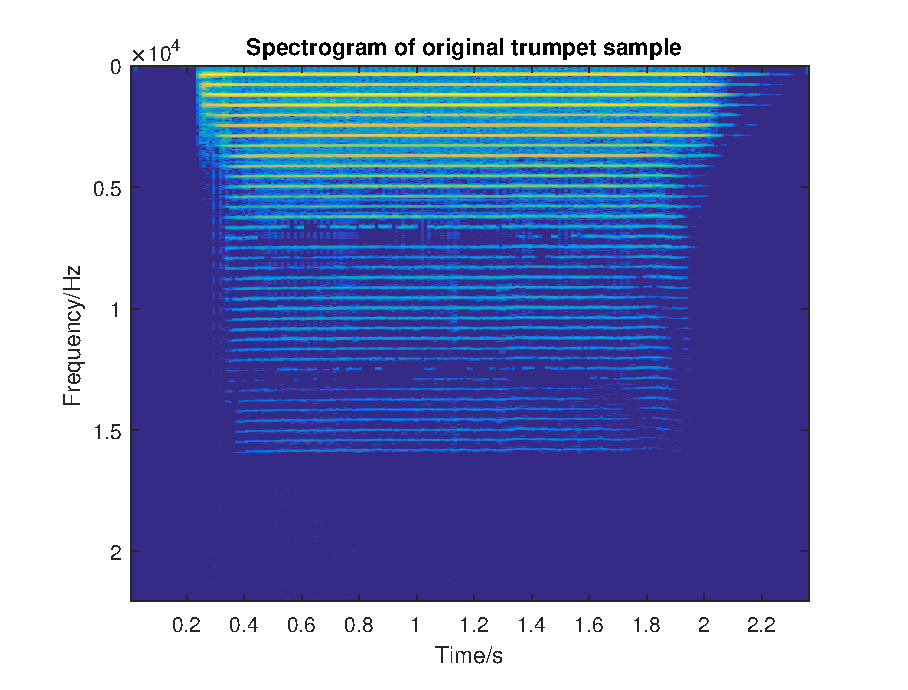
\includegraphics[width=0.5\linewidth]{./OriginalTrumpet.eps}

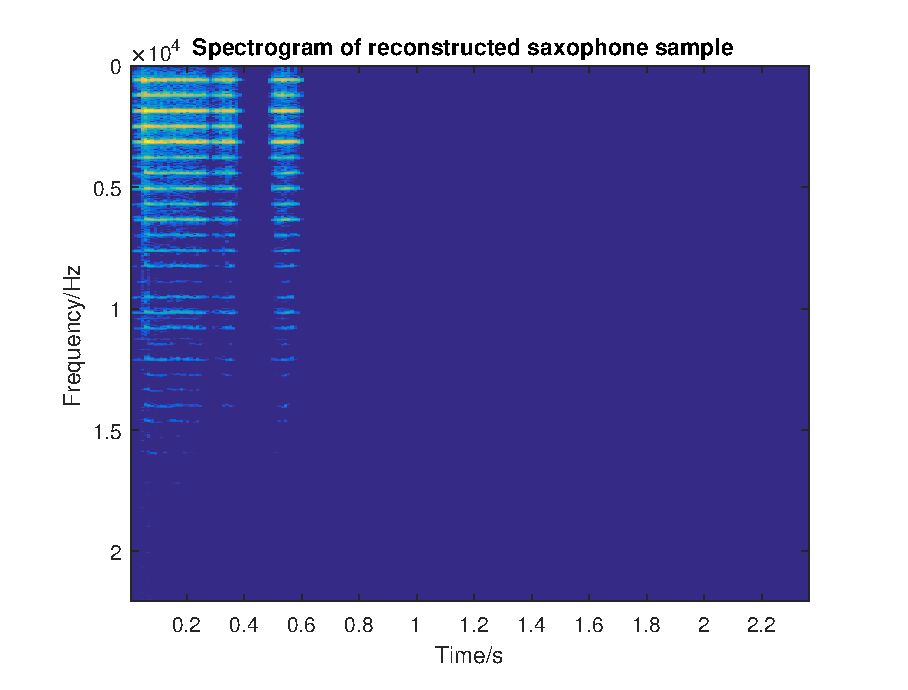
\includegraphics[width=0.5\linewidth]{./ReconstructedSaxophoneNMF10.eps}
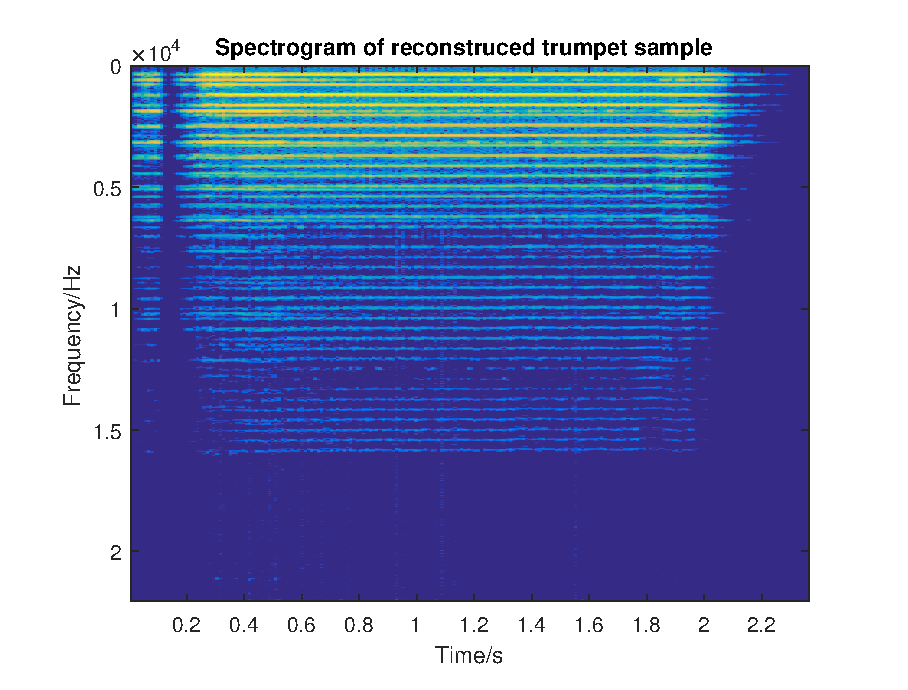
\includegraphics[width=0.5\linewidth]{./ReconstructedTrumpetNMF10.eps}

\end{frame}

\begin{frame}

\frametitle{Example Results: NMF (cont.)}

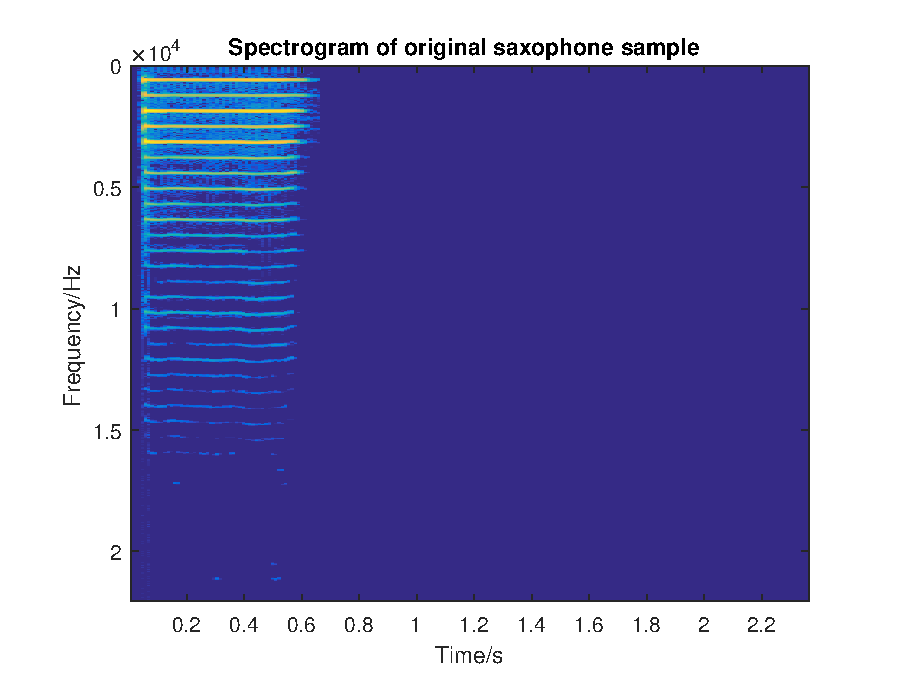
\includegraphics[width=0.5\linewidth]{./OriginalSaxophone.eps}
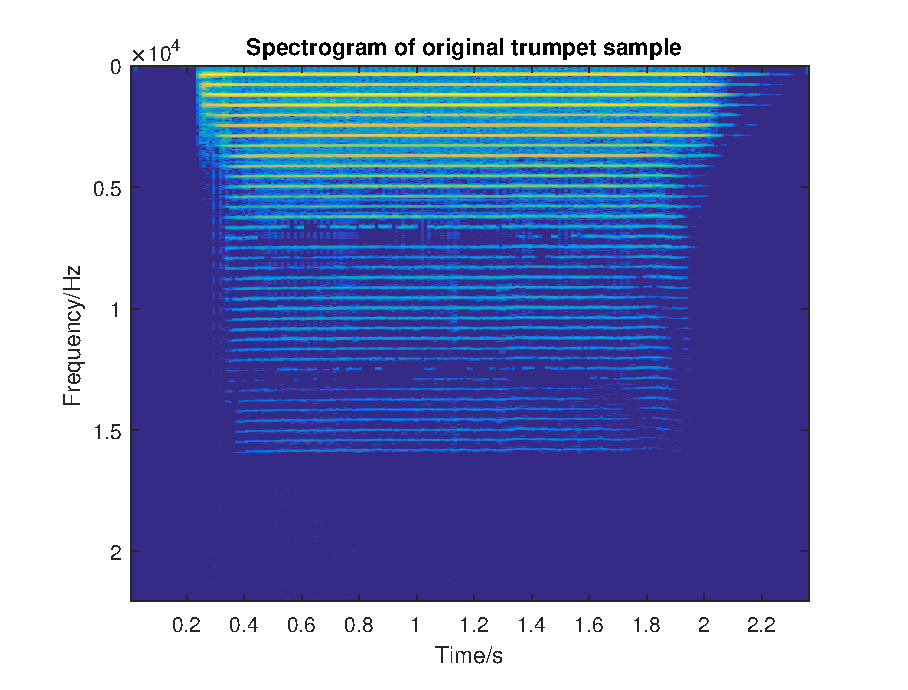
\includegraphics[width=0.5\linewidth]{./OriginalTrumpet.eps}

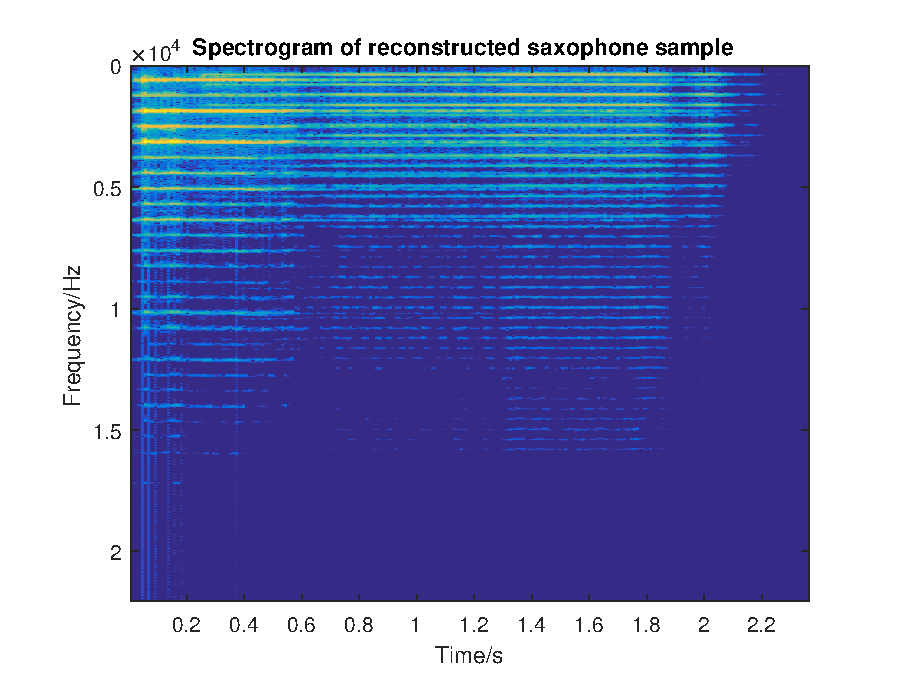
\includegraphics[width=0.5\linewidth]{./ReconstructedSaxophoneNMF100.eps}
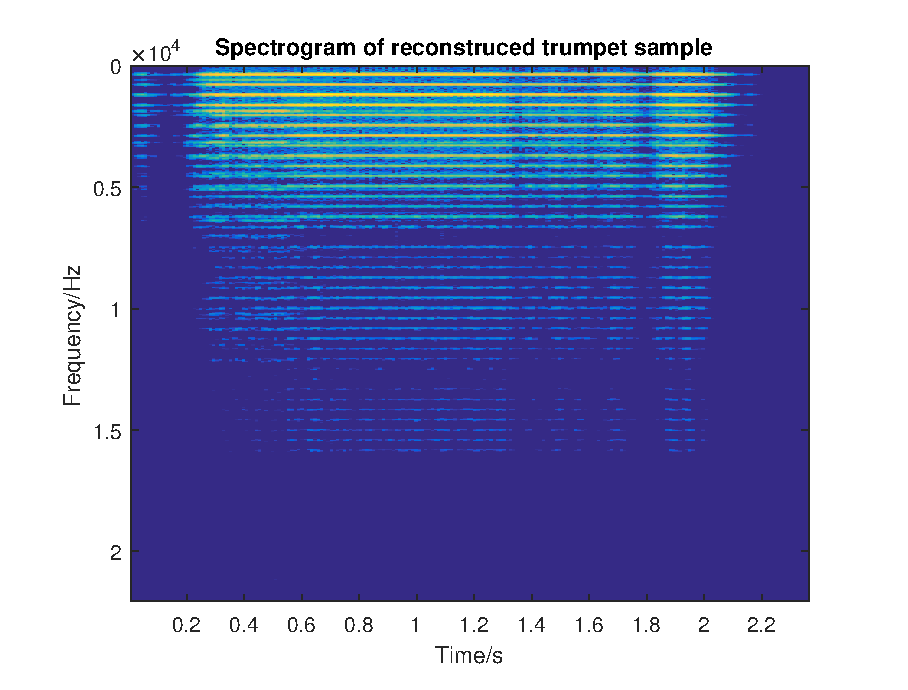
\includegraphics[width=0.5\linewidth]{./ReconstructedTrumpetNMF100.eps}

\end{frame}

\begin{frame}

\frametitle{Example Results: NMF (cont.)}

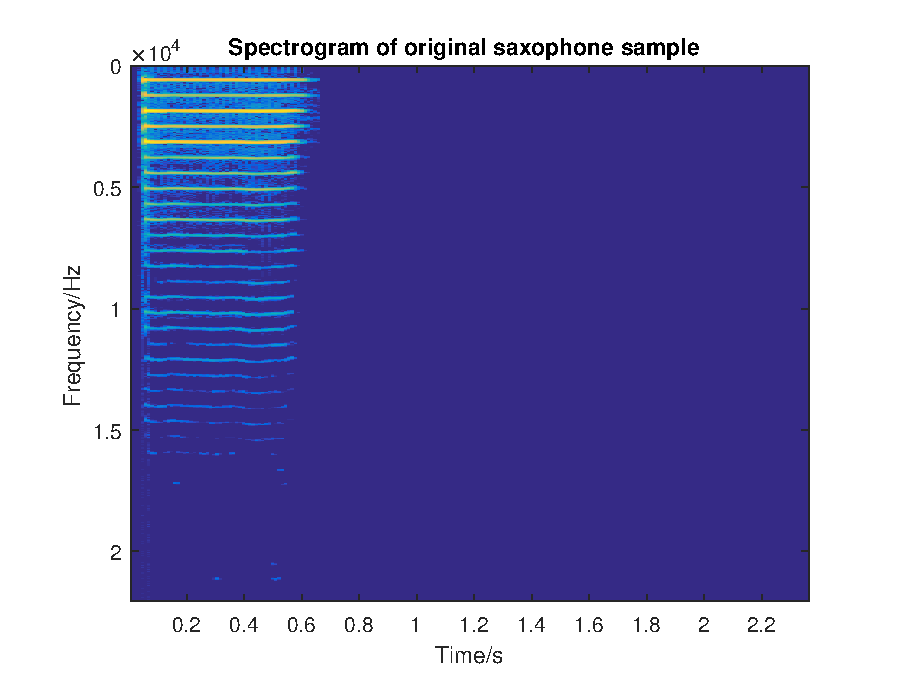
\includegraphics[width=0.5\linewidth]{./OriginalSaxophone.eps}
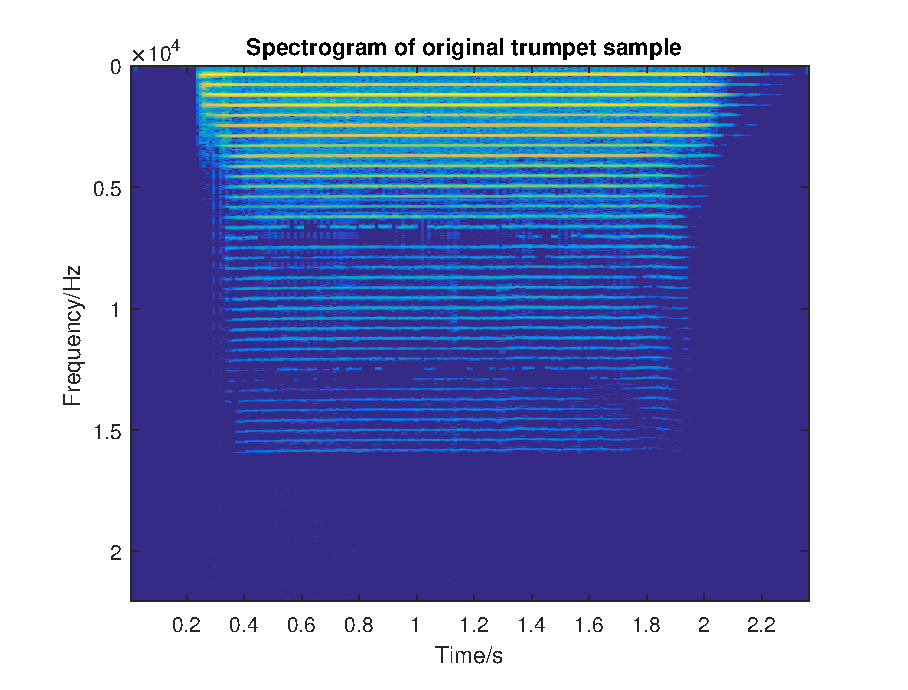
\includegraphics[width=0.5\linewidth]{./OriginalTrumpet.eps}

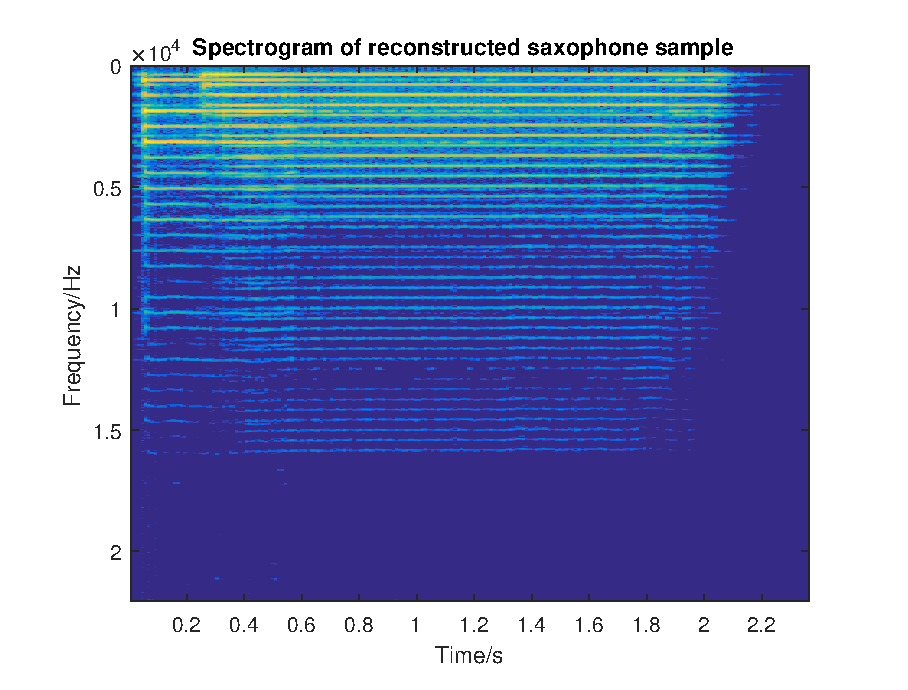
\includegraphics[width=0.5\linewidth]{./ReconstructedSaxophoneNMF1000.eps}
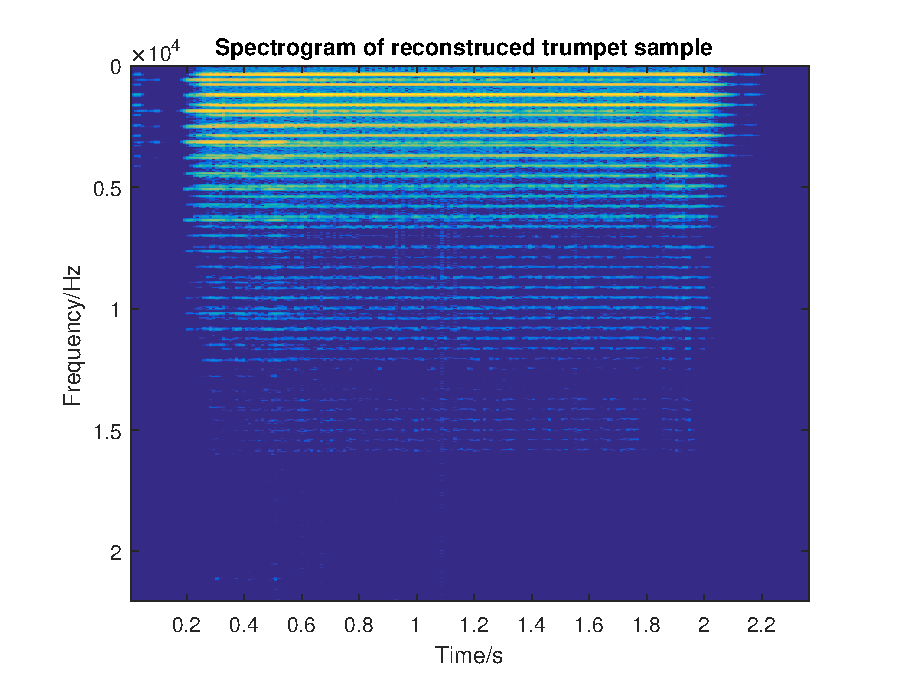
\includegraphics[width=0.5\linewidth]{./ReconstructedTrumpetNMF1000.eps}

\end{frame}

\begin{frame}

\frametitle{Remaining Plans}

Obtain accuracy statistics over various test sets

\bigskip
\bigskip

Further experiments on current solutions

\bigskip
\bigskip

Extension: investigating another separation method

\bigskip
\bigskip

Dissertation

\end{frame}

\begin{frame}

\frametitle{Questions}

\end{frame}

\end{document}